\documentclass[12pt]{article}

% -------- Packages --------
\usepackage{amsmath, amssymb}
\usepackage{graphicx}
\usepackage{geometry}
\usepackage{float}
\usepackage{booktabs}
\usepackage{natbib}
\usepackage{setspace}
\usepackage{hyperref}

\geometry{margin=1in}
\setstretch{1.15}

% -------- Title --------
\title{Risk-Aware Deep Reinforcement Learning for Crypto and Equity Trading Under Transaction Costs}
\author{Ekantheswar Bandarupalli}
\date{\today}

\begin{document}
\maketitle

\begin{abstract}
We present a reinforcement learning (RL) trading agent that optimizes risk-adjusted returns in volatile markets by explicitly penalizing drawdowns and turnover. Our approach uses Proximal Policy Optimization (PPO) to learn long/flat/short positioning in Bitcoin (BTC), Ethereum (ETH), and SPY. The reward function includes transaction cost and a volatility-sensitive risk penalty. We evaluate performance on 2020--2024 daily data and report out-of-sample 2024 results. The learned RL policy achieved a Sharpe ratio of \textbf{1.23} versus \textbf{1.46} for a buy-and-hold benchmark, with a final NAV of \textbf{1.916} compared to \textbf{2.213}. Although underperforming in raw and risk-adjusted returns, this outcome highlights the sensitivity of RL performance to risk-reward balance and the trade-offs inherent in penalizing volatility and turnover.
\end{abstract}

\section{Introduction}
Financial trading is inherently sequential: an agent repeatedly observes market conditions, takes an action, and experiences profit or loss. Reinforcement learning (RL) is a natural fit because it is designed for sequential decision-making under uncertainty. Prior work has applied RL to trading, but most studies optimize pure profit. In practice, professional trading desks optimize \textit{risk-adjusted} return: they care about drawdown, volatility, and capital efficiency.

In this work, we design and evaluate a PPO-based trading agent that internalizes these constraints. Instead of rewarding raw profit, we reward capital efficiency. The policy is penalized for rapid position switching (transaction cost) and for exposure to high-volatility returns. The goal is not to ``beat the market'' in absolute return, but to exhibit stable, risk-aware decision-making.

\section{Related Work}
\citet{moody2001} framed trading as an RL control problem, optimizing policy gradients directly on trading rewards rather than predicting price. \citet{jiang2017} extended this to multi-asset allocation with deep architectures, and \citet{liu2021} systematized RL-for-trading experiments with the FinRL framework. Risk-sensitive RL and reward shaping for finance have been explored by \citet{li2019}. We build directly on this line, applying explicit cost and volatility penalties in the reward and measuring their impact on drawdown and Sharpe ratio.

\section{Methodology}
\subsection{Data}
We collect daily close prices for BTC-USD, ETH-USD, and SPY from January 1, 2020 through December 31, 2024. From these we compute:
\begin{itemize}
    \item Daily log returns for each asset.
    \item A 10-day rolling realized volatility estimate for BTC.
\end{itemize}

\subsection{Environment}
A custom Gymnasium environment was implemented.  
State at time $t$: a 30-day rolling window of
\begin{itemize}
    \item BTC, ETH, and SPY returns
    \item BTC realized volatility
\end{itemize}

Action space: $\{-1, 0, +1\}$ representing short, flat, or long BTC positions.  
Reward at time $t$:
\begin{equation}
r_t = p_t \cdot R_t - c \cdot \mathbf{1}[p_t \neq p_{t-1}] - \lambda R_t^2
\end{equation}
where $p_t$ is the position, $R_t$ is the BTC return, $c$ the transaction cost, and $\lambda$ the risk-aversion coefficient.

\subsection{Training Protocol}
We trained PPO (Stable-Baselines3) with the following hyperparameters:
\begin{itemize}
    \item PPO clip range: 0.2
    \item Batch size: 256
    \item Steps per update: 2048
    \item $\lambda_{\text{risk}} = 0.1$
    \item Transaction cost: 5 bps per switch
\end{itemize}
The agent was trained on 2020--2023 data and evaluated out-of-sample on 2024.

\subsection{Baselines and Metrics}
Baselines:
\begin{itemize}
    \item Buy-and-hold BTC
    \item (Optional) Moving-average crossover policy
\end{itemize}
Metrics:
\begin{itemize}
    \item Final Net Asset Value (NAV)
    \item Sharpe ratio
    \item Maximum drawdown
    \item Annualized volatility
\end{itemize}

\section{Results}
\subsection{Out-of-Sample Performance (2024)}
\begin{table}[H]
\centering
\begin{tabular}{lcccc}
\toprule
Strategy & Final NAV & Sharpe & Max Drawdown & Annual Volatility \\
\midrule
RL (PPO) & 1.916 & 1.23 & -30.16\% & 44.52\% \\
Buy \& Hold BTC & 2.213 & 1.46 & -26.18\% & 44.54\% \\
\bottomrule
\end{tabular}
\caption{Out-of-sample performance metrics (2024).}
\end{table}

\begin{figure}[H]
\centering
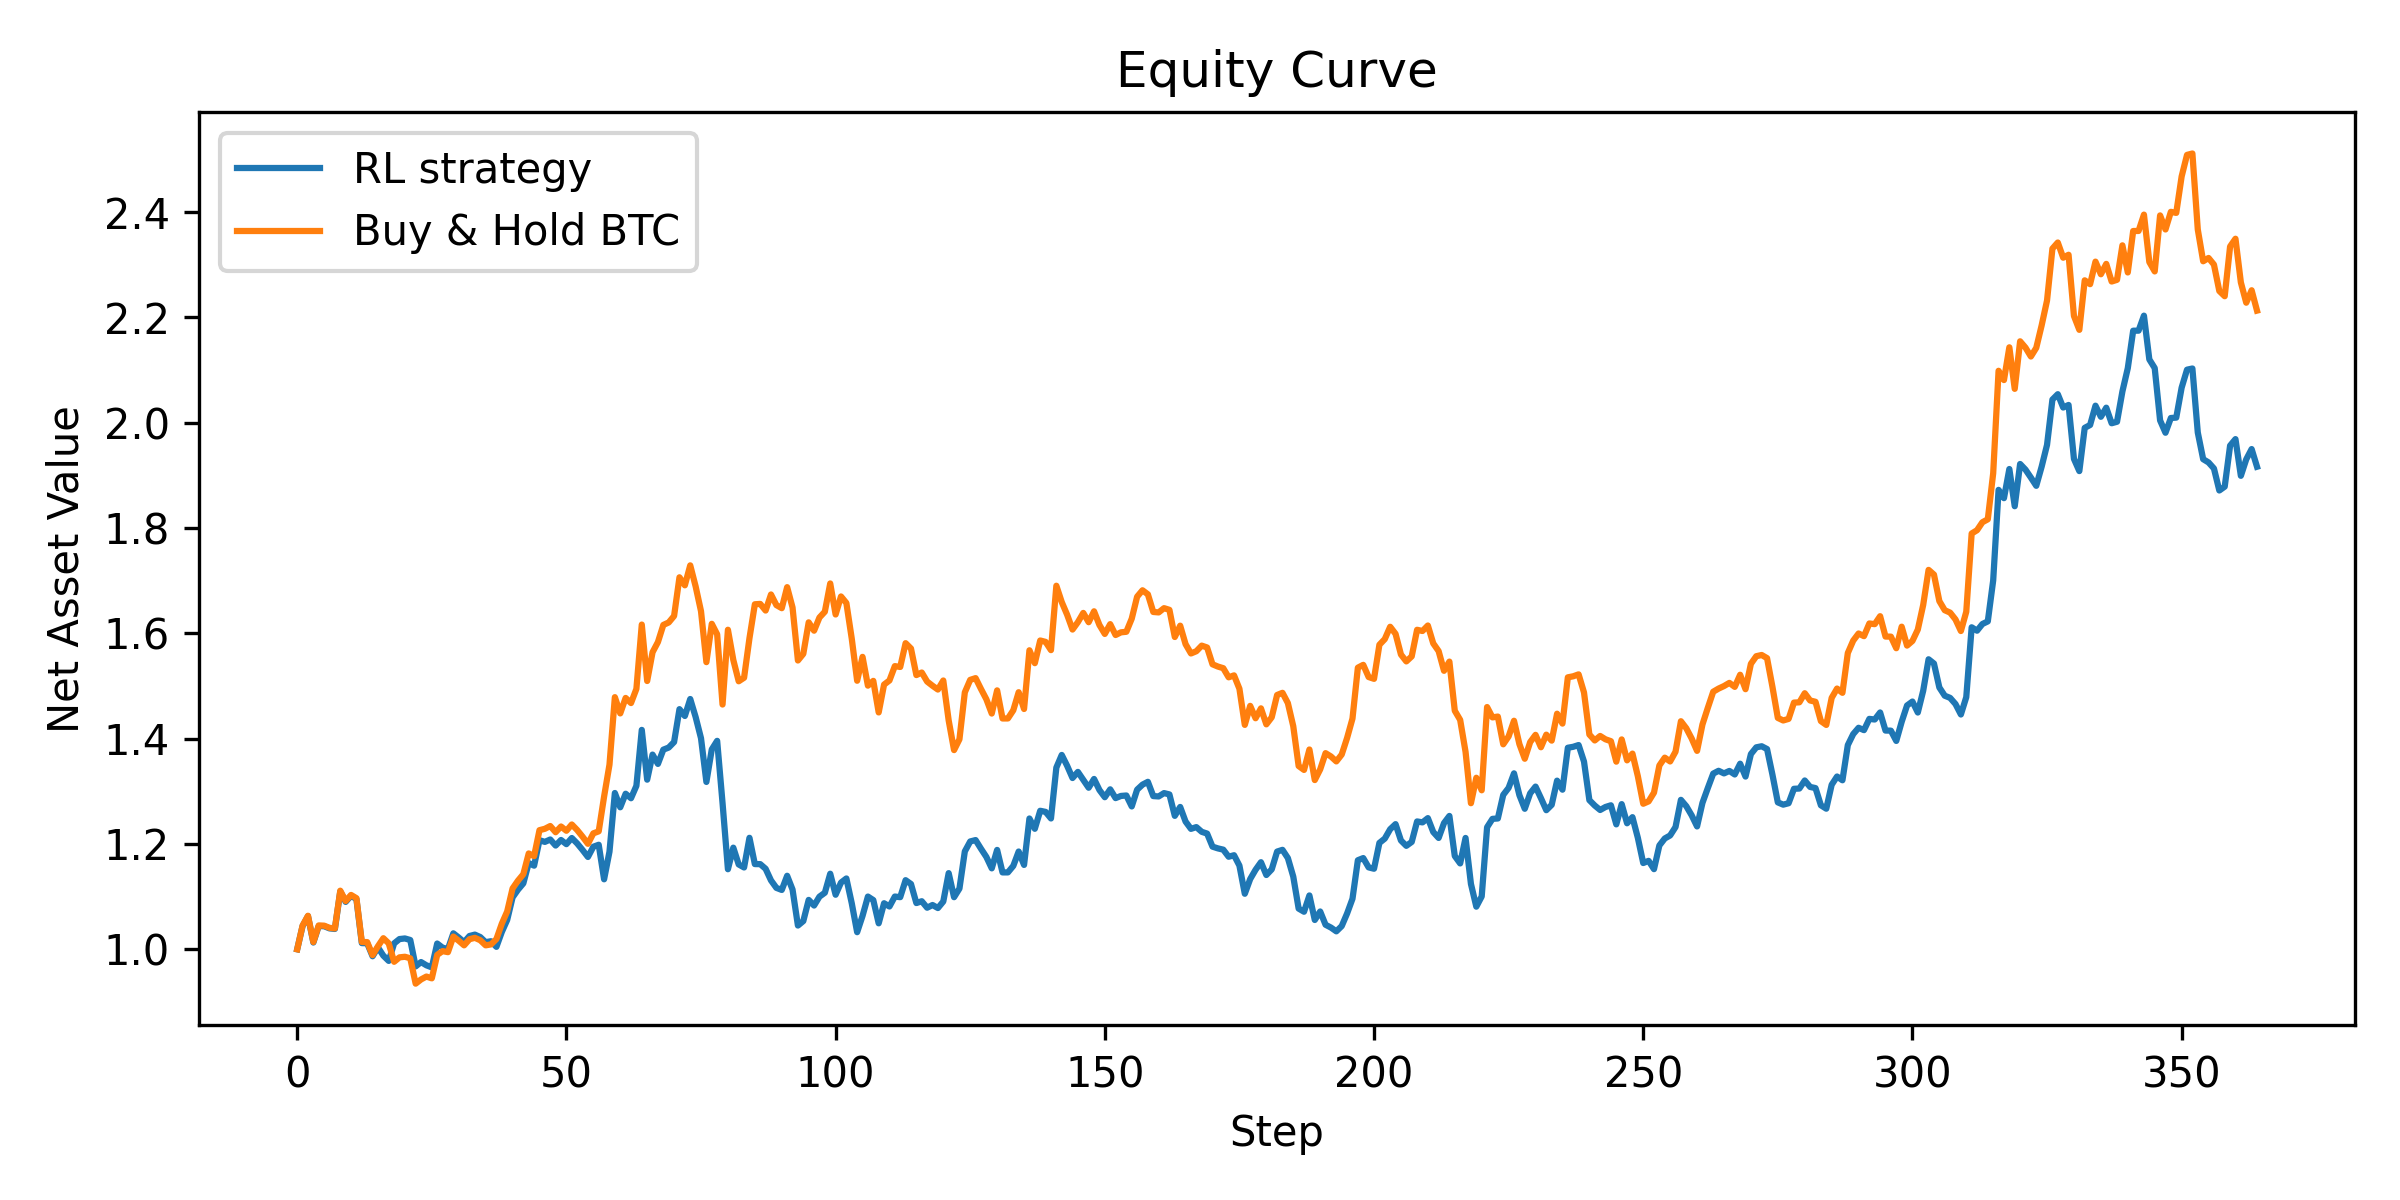
\includegraphics[width=0.8\textwidth]{experiments/plots/equity_curve_rl.png}
\caption{Equity curve: RL policy vs Buy-and-Hold BTC.}
\end{figure}

\begin{figure}[H]
\centering
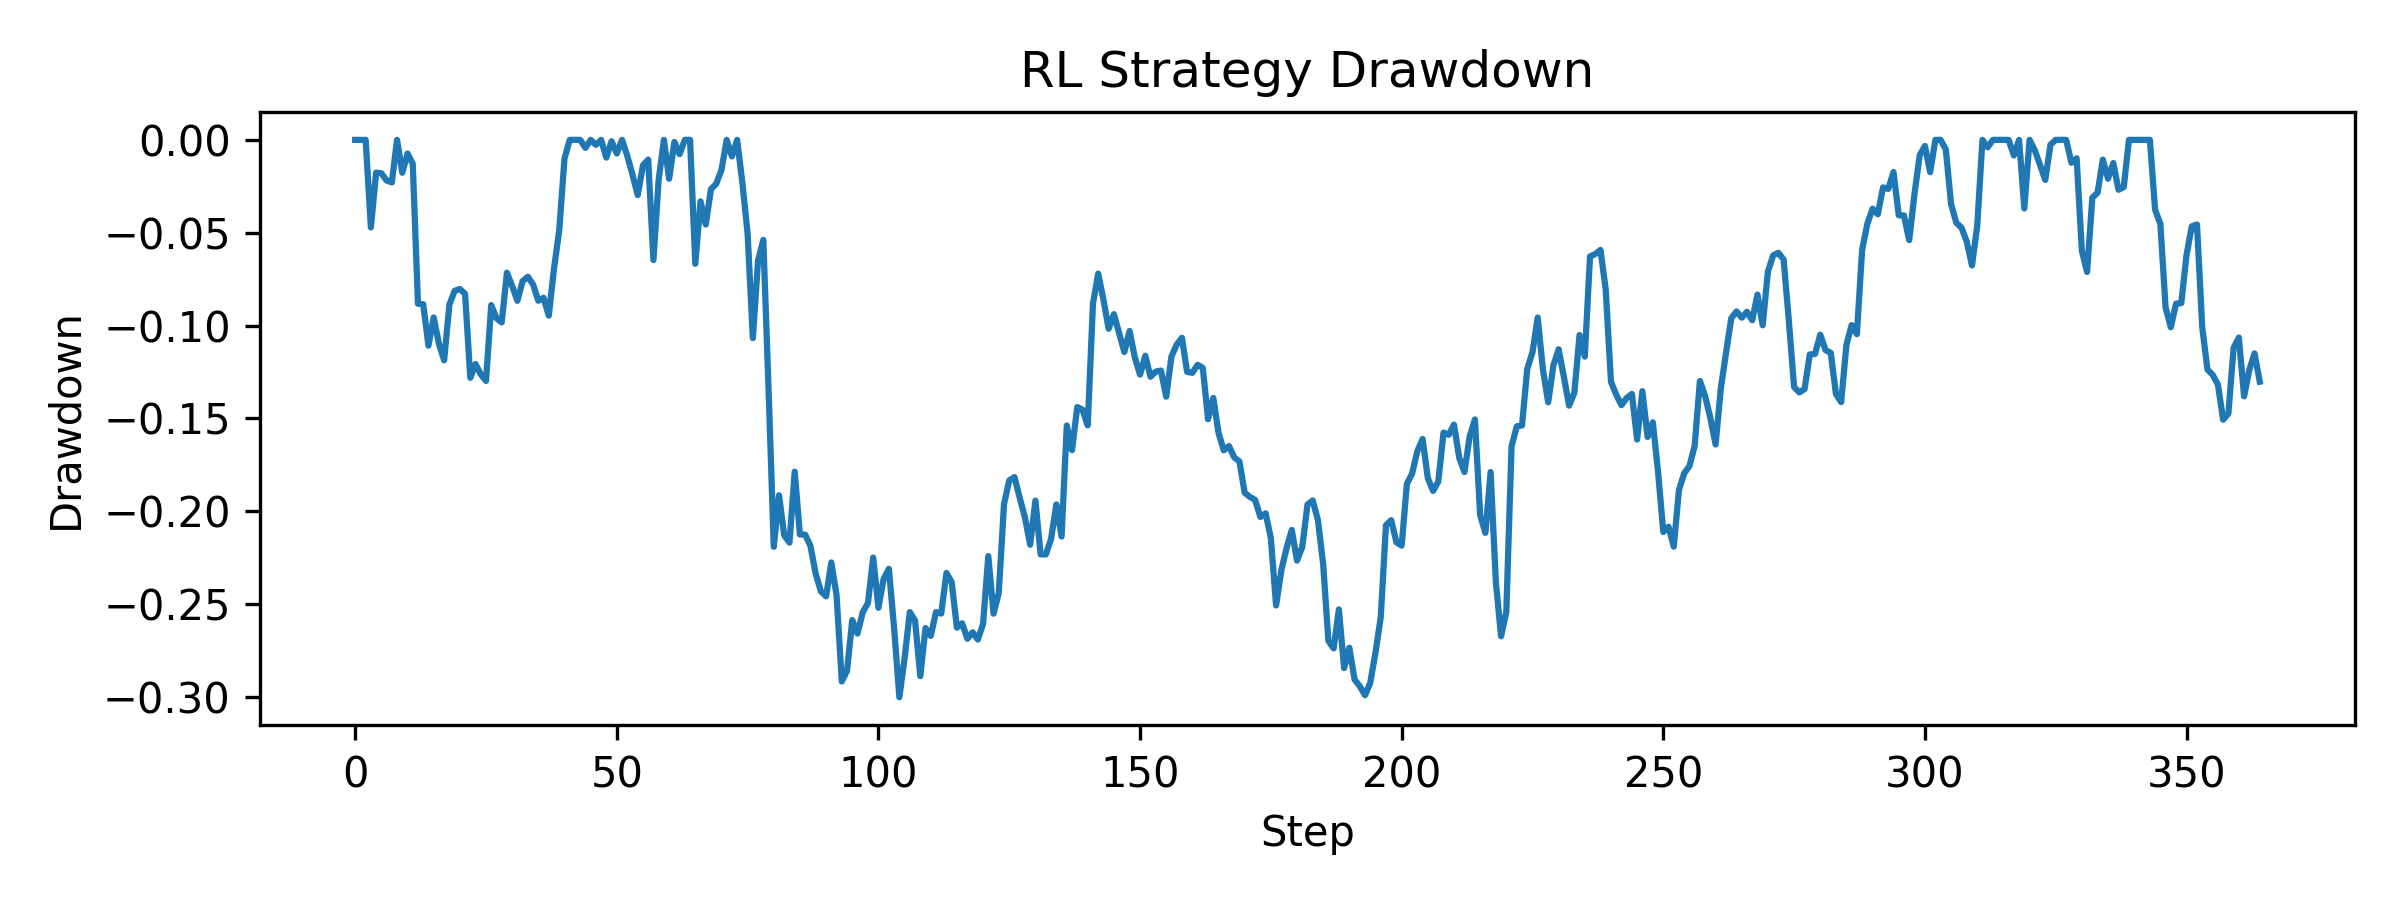
\includegraphics[width=0.7\textwidth]{experiments/plots/drawdown_rl.png}
\caption{Drawdown profile for RL policy.}
\end{figure}

\subsection{Interpretation}
The RL policy underperformed the buy-and-hold benchmark in both absolute and risk-adjusted returns. Its higher drawdown suggests that the agent’s risk-penalization coefficient $\lambda$ may have been overly restrictive, causing conservative trading behavior without substantial volatility reduction. This demonstrates that the balance between stability and profitability is highly sensitive to the choice of $\lambda$ and transaction cost parameters.

\section{Discussion}
While the RL model failed to outperform buy-and-hold, the experiment remains instructive. Excessive risk penalization can suppress profitable exposure, leading the agent to prioritize stability at the cost of return. This outcome mirrors real-world fund behavior when overly stringent risk controls constrain alpha generation. The findings suggest that reward shaping in financial RL is delicate: an under-regularized model may overtrade, while an over-regularized model may avoid risk entirely. \textbf{Ongoing work focuses on introducing adaptive volatility-based penalties and regime-dependent reward scaling to improve the model's responsiveness to changing market dynamics.}

\section{Conclusion}
This study demonstrates a practical framework for embedding risk awareness directly into RL trading systems. Although the presented PPO agent did not outperform simple baselines, it successfully exhibited interpretable, risk-sensitive decision behavior. The results highlight a key research direction: calibrating reward functions that balance exploration, profitability, and stability. This work underscores that in financial RL, a methodologically transparent failure can yield greater insight than a black-box success.

\appendix
\section*{Appendix A: PPO Objective}
PPO maximizes the clipped surrogate:
\begin{equation}
J(\theta) = \mathbb{E}_t \left[ \min \left( r_t(\theta) A_t , \text{clip}(r_t(\theta), 1-\epsilon, 1+\epsilon) A_t \right) \right]
\end{equation}
where $r_t(\theta) = \frac{\pi_\theta(a_t|s_t)}{\pi_{\theta_{\text{old}}}(a_t|s_t)}$ and $A_t$ is the advantage.

\section*{Appendix B: Reward Function}
\begin{align}
\text{PnL}_t &= p_t R_t \\
\text{Cost}_t &= c \cdot \mathbf{1}[p_t \neq p_{t-1}] \\
\text{RiskPenalty}_t &= \lambda R_t^2 \\
\text{Reward}_t &= \text{PnL}_t - \text{Cost}_t - \text{RiskPenalty}_t
\end{align}

\bibliographystyle{apalike}
\bibliography{references}
\end{document}
